\subsubsection*{\textit{Explanation of Simulation-Based Models}}

A Simulator-Based model is a parameterized stochastic data generating
mechanism \autocite{Gutmann2016}. The key characteristic is that
although we are able to sample (simulate) data points, we cannot
evaluate the likelihood for a specific set of observations
$\data$. Formally, a simulator-based model is described as a
parameterized family of probability density functions
$\{ p_{\yb|\thetab}(\yb) \}_{\thetab}$, whose closed-form is either
unknown or intractable to evaluate. Although, evaluating
$p_{y|\theta}(y)$ is intractable, sampling is feasible. Practically, a
simulator can be understood as a black-box machine $M_r$\footnote{The
  subscript $r$ in $M_r$ indicates the \textit{random} simulator. In
  the next chapters we will introduce $M_d$ witch stands for the
  \textit{deterministic} simulator.} that, given parameter $\thetab$,
produces samples $\yb$ in a stochastic manner, i.e.\
$M_r(\thetab) \rightarrow \yb$.

Simulator-Based models are particularly captivating due to the
low-level of restrictions they demand in the modeling; any physical
process that can be conceptualized as a computer program of finite
(determinstic or stochastic) steps, can be modelled as a
Simulator-Based model without any mathematical compromise. This
includes any amount of hidden (unobserved) internal variables or
logic-based decisions. On the other hand, this level of freedom comes
at a cost; performing inference is particularly demanding from both
computational and mathematical perspective. Unfortunately, the
algorithms deployed so far, allow the performance of inference only at
low-dimensionality parametric spaces, i.e.\ $\thetab \in \mathbb{R}^D$
where $D$ is small.

\subsubsection*{\textit{Example}}

For illustrating the importance of Simulator-Based models, lets use
the tuberculosis disease spread example as described in
\autocite{Tanaka2006}. At each stage one of the following
\textit{unobserved} events may happen; (a) the transmission of a
specific haplotype to a new host (b) the mutation to a different
haplotype (c) the exclusion of an infectius host (recovers/dies). The
random process, which stops when $m$ infectius hosts are reached, can
be parameterized (a) by the transmission rate $\alpha$ (b) the
mutation rate $\tau$ and (c) the exclusion rate $\delta$, creating a
$3D$-parametric space $\thetab = (\alpha, \tau, \delta)$. The outcome
of the process is a variable-sized tuple $\yb_{\thetab}$, containg the
size of all different infection groups, as described in
figure~\ref{fig:tuberculosis_model}. Computing $p(\yb=\data|\thetab)$
requires tracking all tree-paths that generate the specific tuple
along with their probabilities and summing over them. Computing this
probability becomes intractable when $m$ grows larger as in real-case
scenarios. On the other hand, modeling the data-generation process as
a computer program is simple and computationally efficient, hence
using a Simulator-Based Model is a perfect fit.

\begin{figure}[!ht]
    \begin{center}
      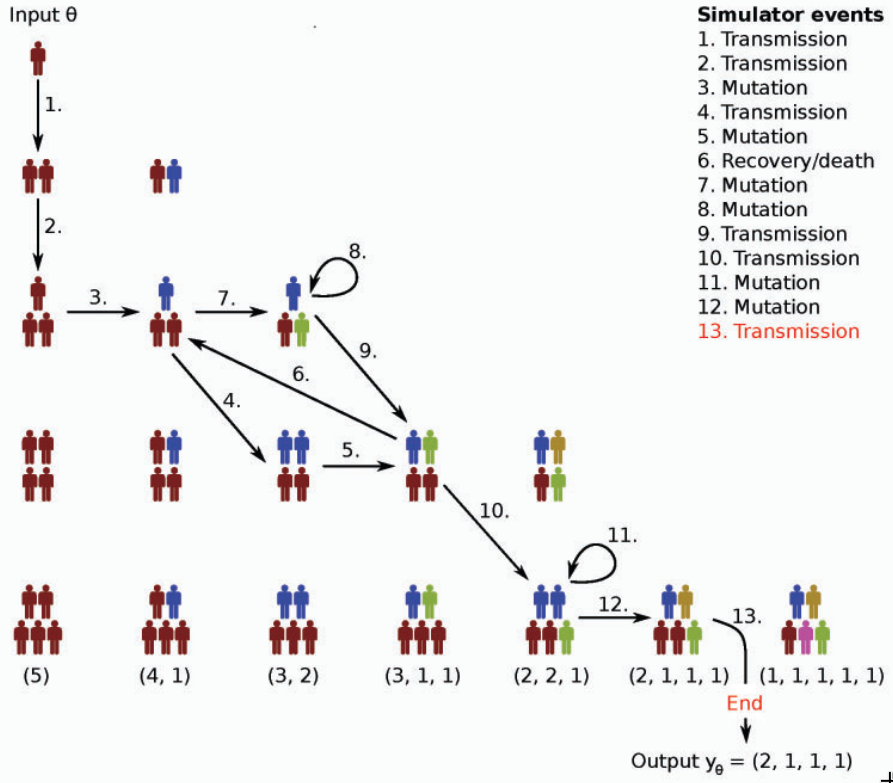
\includegraphics[width=0.75\textwidth]{./images/chapter1/tuber_model_1.png}
    \end{center}
    \caption{Image taken from \autocite{Lintusaari2017}}
    \label{fig:tuberculosis_model}
\end{figure}

\subsubsection*{\textit{Goal of Simulation-Based Models}}

As in most Machine Learning (ML) concepts, the fundamental goal is the
derivation of one(many) parameter configuration(s) $\thetab^*$ that
\textit{describe} well the data i.e.\ generate samples
$M_r(\thetab^*)$ that are as close as possible to the observed data
$\data$. In our case, following the approach of Bayesian Machine
Learning, we treat the parameters of interest $\thetab$ as random
variables and we try to \textit{infer} a posterior distribution
$p(\thetab|\data)$ on them. 

\subsubsection*{\textit{Robust Optimisation Monte Carlo (ROMC) method}}

The ROMC method \autocite{Ikonomov2019} is very a recent Likelihood-Free
approach; its fundamental idea is the transformation of the stochastic
data generation process $M_r(\thetab)$ to a deterministic mapping
$g_i(\thetab)$, by pre-sampling the variables that produce the randomness
$\vb_i \sim p(\V)$. Formally, in every stochastic process the randomness
is influenced by a vector of random variables $\vb$, whose state is
unknown before the execution of the simulation; pre-sampling this
state makes the procedure deterministic, namely
$g_i(\thetab) = M_d(\thetab, \V=\vb_i)$. This approach initially introduced
at \autocite{Meeds2015} with the title \textit{Optimisation Monte
Carlo (OMC)}. The ROMC extended this approach by resolving a
fundamental failure-mode of OMC. The ROMC describes a methodology for
approximating the posterior through a series of steps, without
explicitly enforcing which algorithms must be used for each
step\footnote{The implementation chooses a specific algorithm for each
  task, but this choice has just a demonstrative value; any other
  appropriate algorithm can be used instead.}; in this sense it can be
thought as a meta-algorithm.

\subsubsection*{\textit{Implementation}}

The most important contribution of this work is the implementation of
the ROMC method in the Python package Engine for Likelihood-Free
Inference (ELFI) \autocite{1708.00707}. Since it is very recently
published work the ROMC method was not implemented by now in any ML
software. This works attempts to provide to the research community a
tested and robust implementation for further experimentation and
possible extensions.
